\problemname{Tingsplatsen}

Arkeologen Arvid är på jakt efter en okänd tingsplats från järnåldern någonstans i Mellansverige. Han har kartlagt
ett antal gårdar som fanns i området, och har kommit fram till att tingsplatsen måste ligga på samma avstånd
till de olika gårdarna.

Området som Arvid undersökt kan representeras av ett rutnät med $N$ rader och $M$ kolumner. Det tar en minut för en
järnåldersmänniska att ta sig mellan två närliggande rutor. Två rutor är närliggande om de delar en av sina fyra sidor.
Du får givet en karta av rutnätet som markerar var de olika gårdarna som Arvid undersökt är. Det är känt att det tar lika
lång tid att ta sig från var och en av gårdarna till den okända tingsplatsen. Din uppgift är att hitta vilka rutor där
tingsplatsen skulle kunna finnas.

\section*{Indata}
Den första raden består av två heltal $N$ och $M$ ($1 \leq N,M \leq 10$), antalet rader och kolumner i rutnätet.

De följande $N$ raderna innehåller vardera en sträng av längd $M$, som består av tecknen ''\verb|.|'' och ''\verb|*|''.
Det här är raderna i rutnätet. Tecknet ''\verb|*|'' betyder att det finns en gård på motsvarande plats i rutnätet, och
''\verb|.|'' betyder att det inte finns en gård.

Det kommer finnas minst två gårdar i rutnätet. Indatan har genererats på så sätt att det alltid finns minst en ruta där tingsplatsen kan vara.

\section*{Utdata}
Skriv ut $N$ rader med en sträng av längd $M$ på varje rad, en kopia av rutnätet i indatan men där du markerat med ''\verb|X|''
 de rutor som tingsplatsen kan vara belägen på.

\section*{Poängsättning}
Din lösning kommer att testas på en mängd testfallsgrupper.
För att få poäng för en grupp så måste du klara alla testfall i gruppen.

\noindent
\begin{tabular}{| l | l | p{12cm} |}
  \hline
  \textbf{Grupp} & \textbf{Poäng} & \textbf{Gränser} \\ \hline
  $1$    & $20$  & $N = 1$ \\ \hline
  $2$    & $80$  & Inga ytterligare begränsningar. \\ \hline
\end{tabular}

\section*{Förklaring av exempelfall}

\begin{figure}[h]
  \centering
  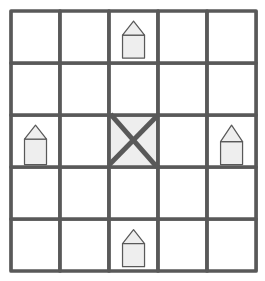
\includegraphics[width=0.2\textwidth]{sample3.png}
    \\Bilden visar lösningen till exempelfall 3. Den markerade rutan i mitten är den enda möjliga positionen hos tingsplatsen.
    Det tar två minuter att ta sig från varje gård till den här rutan.
  
\end{figure}
